
\documentclass[10pt,aspectratio=43]{beamer}

\usepackage{ctex}
\usepackage{fontspec}
\IfFileExists{C:/Users/Albert/AppData/Local/Microsoft/Windows/Fonts/LXGWWenKai-Regular.ttf}{%
  \setCJKmainfont[
    Path={C:/Users/Albert/AppData/Local/Microsoft/Windows/Fonts/},
    UprightFont={LXGWWenKai-Regular.ttf},
    BoldFont={LXGWWenKai-Regular.ttf}
  ]{LXGW WenKai}
  \setCJKsansfont[
    Path={C:/Users/Albert/AppData/Local/Microsoft/Windows/Fonts/},
    UprightFont={LXGWWenKai-Regular.ttf},
    BoldFont={LXGWWenKai-Regular.ttf}
  ]{LXGW WenKai}
  \newCJKfontfamily\kaifont[
    Path={C:/Users/Albert/AppData/Local/Microsoft/Windows/Fonts/},
    UprightFont={LXGWWenKai-Regular.ttf},
    BoldFont={LXGWWenKai-Regular.ttf}
  ]{LXGW WenKai}
}{%
  \setCJKmainfont{Microsoft YaHei}
  \setCJKsansfont{Microsoft YaHei}
  \newCJKfontfamily\kaifont{KaiTi}
}

\usetheme{Frankfurt}
\usecolortheme{default}

\definecolor{ZJUBlue}{RGB}{0,63,127}
\definecolor{Ink}{RGB}{36,42,49}
\definecolor{SoftBlue}{RGB}{232,240,250}
\definecolor{SoftGreen}{RGB}{236,243,250}
\definecolor{SoftCyan}{RGB}{228,244,247}
\definecolor{SoftSlate}{RGB}{238,243,248}
\definecolor{AccentRed}{RGB}{176,42,55}
\definecolor{AccentGray}{RGB}{90,96,105}
\definecolor{ModelBlue}{RGB}{43,105,168}
\definecolor{AgentGreen}{RGB}{78,112,145}
\definecolor{SignalTeal}{RGB}{36,132,135}

\setbeamercolor{normal text}{fg=Ink,bg=white}
\setbeamercolor{structure}{fg=ZJUBlue}
\setbeamercolor{palette primary}{bg=ZJUBlue,fg=white}
\setbeamercolor{palette secondary}{bg=ZJUBlue!85,fg=white}
\setbeamercolor{palette tertiary}{bg=ZJUBlue,fg=white}
\setbeamercolor{title}{fg=ZJUBlue}
\setbeamercolor{frametitle}{bg=ZJUBlue,fg=white}
\setbeamercolor{block title}{bg=ZJUBlue,fg=white}
\setbeamercolor{block body}{bg=SoftBlue,fg=Ink}
\setbeamerfont{frametitle}{size=\large,series=\bfseries}
\setbeamerfont{title}{size=\Large,series=\bfseries,family=\kaifont}
\setbeamertemplate{navigation symbols}{}
\setbeamertemplate{itemize item}{\color{ZJUBlue}\textbullet}
\setbeamertemplate{itemize subitem}{\color{ZJUBlue!70}\textendash}

\setbeamerfont{section in head/foot}{size=\scriptsize,series=\bfseries}
\setbeamerfont{subsection in head/foot}{size=\tiny}

\setbeamertemplate{footline}{%
  \leavevmode%
  \hbox{%
    \begin{beamercolorbox}[wd=.52\paperwidth,ht=2.4ex,dp=0.9ex,leftskip=1em]{palette primary}
      \scriptsize A股预测中期报告
    \end{beamercolorbox}%
    \begin{beamercolorbox}[wd=.48\paperwidth,ht=2.4ex,dp=0.9ex,rightskip=1em]{palette primary}
      \hfill\scriptsize \Acrobatmenu{PrevPage}{\textcolor{white}{$\leftarrow$}}\hspace{0.35em}
      \Acrobatmenu{NextPage}{\textcolor{white}{$\rightarrow$}}\hspace{0.8em}\insertframenumber{} / \inserttotalframenumber
    \end{beamercolorbox}%
  }%
}

\usepackage{graphicx}
\usepackage{tikz}
\usepackage{booktabs}
\usepackage{array}
\usepackage{pifont}
\usepackage{tcolorbox}
\usepackage{colortbl}
\usepackage{amsmath}
\tcbuselibrary{skins}
\usetikzlibrary{positioning,arrows.meta,shapes.geometric,fit,backgrounds,calc}

\newcommand{\cmark}{\textcolor{ZJUBlue}{\ding{51}}}
\newcommand{\xmark}{\textcolor{AccentRed}{\ding{55}}}
\newcommand{\warn}{\textcolor{SignalTeal}{\ding{115}}}
\newcommand{\code}[1]{\texttt{#1}}

\newtcolorbox{hlbox}[1][]{
  colback=SoftBlue, colframe=ZJUBlue, boxrule=0.55pt,
  arc=2pt, left=6pt,right=6pt,top=4pt,bottom=4pt,
  fonttitle=\bfseries, #1
}
\newtcolorbox{greenbox}[1][]{
  colback=SoftGreen, colframe=ZJUBlue!72, boxrule=0.55pt,
  arc=2pt, left=6pt,right=6pt,top=4pt,bottom=4pt,
  fonttitle=\bfseries, #1
}
\newtcolorbox{orangebox}[1][]{
  colback=SoftCyan, colframe=SignalTeal, boxrule=0.55pt,
  arc=2pt, left=6pt,right=6pt,top=4pt,bottom=4pt,
  fonttitle=\bfseries, #1
}

\title[A股预测]{A股预测中期报告}
\subtitle{从短期价格预测实验到交互式 A 股研究助手}
\author{王昱人 3230105943 \quad 高烁斌 3230101940 \quad 于臻 3230105913}
\institute{团队名称：克劳德老师，我还记得你}
\date{2026年7月13日}

\begin{document}

\begin{frame}[plain]
  \vfill
  \begin{center}
    {\color{ZJUBlue}\rule{0.86\textwidth}{1.2pt}}\\[0.8em]
    {\kaifont\Large\bfseries\color{ZJUBlue}\inserttitle}\\[0.35em]
    {\large\color{AccentGray}\insertsubtitle}\\[0.65em]
    {\color{ZJUBlue}\rule{0.86\textwidth}{1.2pt}}\\[1.8em]
    \begin{tabular}{rl}
      \textbf{课题名称：} & （Mo平台项目）A股预测 \\
      \textbf{团队名称：} & 克劳德老师，我还记得你 \\
      \textbf{成员：} & 王昱人 3230105943\\
      & 高烁斌 3230101940\\
      & 于臻 \, \, 3230105913\\
      \textbf{汇报日期：} & 2026年7月13日
    \end{tabular}
  \end{center}
  \vfill
\end{frame}

\section{结构}

\begin{frame}{汇报结构}
  \vspace{0.3em}
  \begin{columns}[T]
    \begin{column}{0.5\textwidth}
      \begin{hlbox}[title=课程作业主线]
        \small
        \textbf{1.} 问题背景与目标\\[0.35em]
        \textbf{2.} 数据处理与 LSTM 训练\\[0.35em]
        \textbf{3.} 平台结果与局限分析
      \end{hlbox}
    \end{column}
    \begin{column}{0.5\textwidth}
      \begin{greenbox}[title=系统扩展主线]
        \small
        \textbf{4.} 投资助手 Agent 架构\\[0.35em]
        \textbf{5.} 工具体系与问答测试\\[0.35em]
        \textbf{6.} 问题、改进与结题计划
      \end{greenbox}
    \end{column}
  \end{columns}
  \vspace{0.9em}
  \begin{center}
    {\kaifont\large\color{ZJUBlue}将LSTM 短期预测作为投资助手中的一个量化工具}
  \end{center}
\end{frame}

\section{课程作业}

\begin{frame}{课题背景与目标}
  \begin{columns}[T]
    \begin{column}{0.55\textwidth}
      \begin{hlbox}[title=课程任务]
        \footnotesize
        输入某只股票连续 14 天收盘价，预测第 15 天收盘价，并在 Mo 平台进行评测。
      \end{hlbox}
      \vspace{0.45em}
      \textbf{已完成目标：}
      \begin{itemize}\footnotesize
        \item 完成本地训练与 Mo 平台评测
        \item 对比直接价格预测、MLP 与 LSTM 的稳定性
        \item 增加相对价格、日收益率、均线偏离、波动率、区间位置等特征
        \item 生成训练曲线、测试预测图与平台评测结果
      \end{itemize}
    \end{column}
    \begin{column}{0.45\textwidth}
      \begin{orangebox}[title=为什么要扩展成 Agent]
        \footnotesize
        只依赖 14 天价格序列，模型很容易退化成“明天接近今天”的近似判断。真实涨跌还受资金流、基本面、公告、政策和情绪共同影响。
      \end{orangebox}
      \vspace{0.45em}
      \begin{greenbox}[title=扩展目标]
        \footnotesize
        构建面向 A 股场景的交互式投资助手 Agent：能查行情、看基本面、做筛选与回测、记录持仓偏好，并在需要时调用深度研究流程。
      \end{greenbox}
    \end{column}
  \end{columns}
\end{frame}

\begin{frame}{LSTM：基础知识}
  \vspace{0.3em}
  \begin{hlbox}[title=核心思想]
    \footnotesize
    LSTM（Long Short-Term Memory）是一类循环神经网络，适合处理时间序列。它通过“门控机制”决定哪些历史信息应该保留、哪些噪声应该遗忘。
  \end{hlbox}
  \vspace{0.8em}
  \centering
  \begin{tikzpicture}[
      scale=0.92,
      transform shape,
      every node/.style={font=\scriptsize, align=center},
      cell/.style={draw=ModelBlue!85, fill=SoftBlue, rounded corners=2pt,
                   minimum width=20mm, minimum height=9mm, inner sep=3pt},
      gate/.style={draw=SignalTeal!85, fill=SoftCyan, rounded corners=2pt,
                   minimum width=22mm, minimum height=9mm, inner sep=3pt},
      arr/.style={->, >=Stealth, line width=0.75pt}
  ]
    \node[cell] (x) {输入序列\\$x_t$};
    \node[gate, right=8mm of x] (forget) {遗忘门\\forget};
    \node[gate, right=8mm of forget] (input) {输入门\\input};
    \node[gate, right=8mm of input] (output) {输出门\\output};
    \node[cell, below=8mm of input] (state) {隐藏状态\\$h_t$};
    \draw[arr] (x) -- (forget);
    \draw[arr] (forget) -- (input);
    \draw[arr] (input) -- (output);
    \draw[arr] (input) -- (state);
    \draw[arr] (state) -- (output);
  \end{tikzpicture}
  \vspace{0.9em}
  \begin{greenbox}
    \footnotesize
    在本任务中，LSTM 的作用不是简单的预测价格，而是从短期价格窗口中提取趋势、震荡和回撤等时序模式，作为后续 Agent 决策的一项量化输入。
  \end{greenbox}
\end{frame}

\begin{frame}{LSTM：为什么适合做短期价格工具}
  \vspace{0.3em}
  \begin{columns}[T]
    \begin{column}{0.36\textwidth}
      \begin{hlbox}[title=输入]
        \footnotesize
        连续 14 天价格窗口，以及由价格构造出的收益率、均线偏离、波动率和区间位置。
      \end{hlbox}
    \end{column}
    \begin{column}{0.28\textwidth}
      \begin{orangebox}[title=模型]
        \footnotesize
        LSTM 通过门控结构保留短期序列中的趋势、回撤和震荡信息。
      \end{orangebox}
    \end{column}
    \begin{column}{0.30\textwidth}
      \begin{greenbox}[title=输出]
        \footnotesize
        下一日收益率参考值，最终换算为第 15 天价格预测。
      \end{greenbox}
    \end{column}
  \end{columns}
  \vspace{1em}
  \centering
  \begin{tikzpicture}[
      every node/.style={font=\scriptsize, align=center},
      cell/.style={draw=ModelBlue!85, fill=SoftBlue, rounded corners=2pt,
                   minimum width=13mm, minimum height=8mm, inner sep=2pt},
      signalbox/.style={draw=SignalTeal!85, fill=SoftCyan, rounded corners=2pt,
                  minimum width=21mm, minimum height=9mm, inner sep=2pt},
      arr/.style={->, >=Stealth, line width=0.7pt}
  ]
    \foreach \x in {1,...,6} {
      \node[cell] (d\x) at (\x*1.35,0) {$t-\x$};
    }
    \node[cell] (d7) at (9.45,0) {$t$};
    \node[signalbox] (lstm) at (5.4,-1.25) {LSTM\\序列记忆};
    \node[signalbox] (pred) at (5.4,-2.55) {$\hat r_{15}$\\收益率预测};
    \foreach \x in {1,...,7} {
      \draw[arr] (d\x) -- (lstm);
    }
    \draw[arr] (lstm) -- (pred);
  \end{tikzpicture}
  \vspace{0.7em}
  \begin{minipage}{0.82\linewidth}
    \centering\scriptsize\color{AccentGray}
    LSTM 为 agent 提供一个可解释的短期量化信号。
  \end{minipage}
\end{frame}

\begin{frame}{LSTM：数据归一化与特征}
  \begin{hlbox}[title=预测目标]
    \footnotesize
    模型不直接输出价格，而是预测下一日收益率残差：
    \[
      r_{15}=\frac{p_{15}}{p_{14}}-1
      \qquad
      \hat p_{15}=p_{14}(1+\alpha\hat r_{15})
    \]
  \end{hlbox}
  \vspace{0.6em}
  \centering
  \begin{tikzpicture}[
      every node/.style={font=\scriptsize, align=center},
      chip/.style={draw=ModelBlue!85, fill=SoftBlue, rounded corners=2pt,
                   minimum width=23mm, minimum height=8mm, inner sep=3pt},
      chip2/.style={draw=SignalTeal!85, fill=SoftCyan, rounded corners=2pt,
                   minimum width=23mm, minimum height=8mm, inner sep=3pt}
  ]
    \node[chip] (f1) {relative price\\相对价格};
    \node[chip, right=3mm of f1] (f2) {daily return\\日收益率};
    \node[chip, right=3mm of f2] (f3) {ma3 deviation\\3日均线偏离};
    \node[chip, right=3mm of f3] (f4) {ma5 deviation\\5日均线偏离};
    \node[chip2, below=5mm of f1] (f5) {rolling std 3\\3日波动率};
    \node[chip2, right=3mm of f5] (f6) {rolling std 5\\5日波动率};
    \node[chip2, right=3mm of f6] (f7) {price position\\区间位置};
    \node[chip2, right=3mm of f7] (f8) {standardization\\训练集统计量};
  \end{tikzpicture}
  \vspace{0.7em}
  \begin{greenbox}
    \footnotesize
    使用方式：每一天被编码成 7 维特征向量，连续 14 天组成一个序列输入 LSTM。特征分别描述价格位置、短期动量、均线偏离和波动环境；推理时复用训练集均值和标准差，避免训练/提交分布不一致。
  \end{greenbox}
\end{frame}

\begin{frame}{LSTM：模型训练}
  \centering
  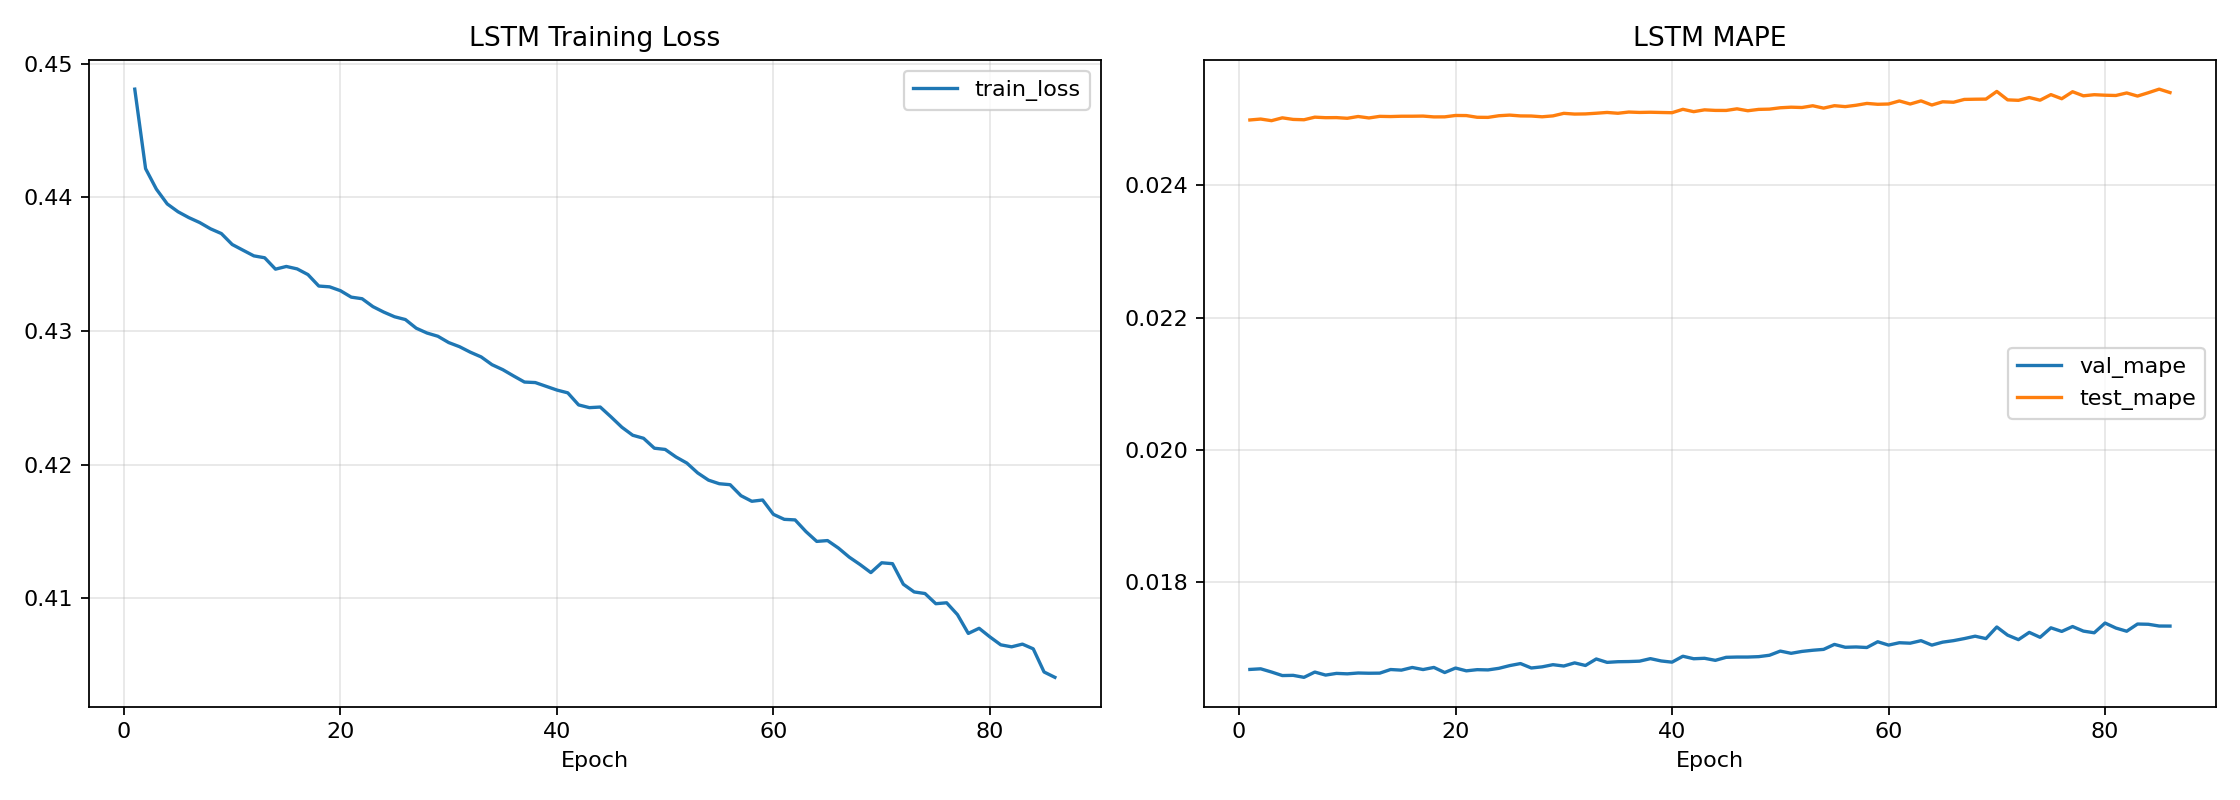
\includegraphics[width=0.97\linewidth]{images/training_curves.png}\\[-0.25em]
  \scriptsize\color{AccentGray}训练/验证损失与 MAPE 曲线
  \vspace{0.35em}
  
  \begin{columns}[T]
    \begin{column}{0.48\textwidth}
      \begin{hlbox}[title=MAPE]
        \scriptsize
        平均绝对百分比误差：
        \[
          \frac{1}{n}\sum_i \left|\frac{y_i-\hat y_i}{y_i}\right|
        \]
      \end{hlbox}
    \end{column}
    \begin{column}{0.48\textwidth}
      \begin{greenbox}[title=MAE]
        \scriptsize
        平均绝对误差：
        \[
          \frac{1}{n}\sum_i |y_i-\hat y_i|
        \]
      \end{greenbox}
    \end{column}
  \end{columns}
\end{frame}

\begin{frame}{LSTM：评测指标与预测效果}
  \centering
  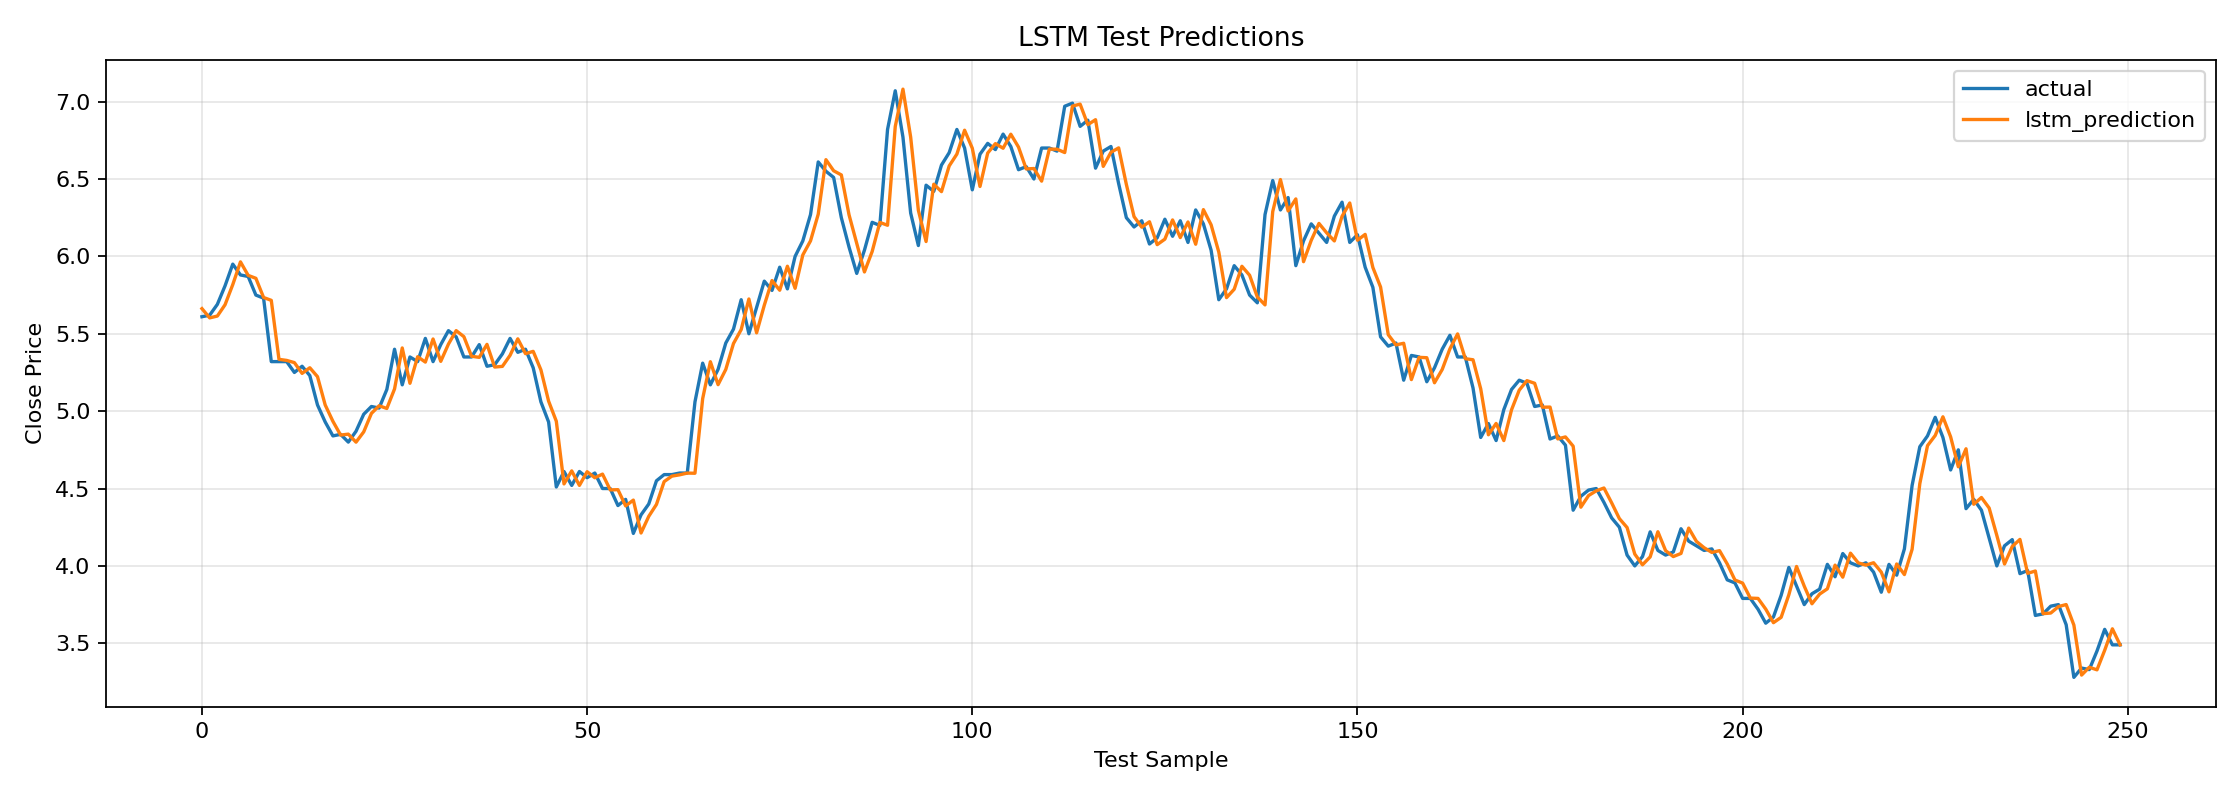
\includegraphics[width=0.96\linewidth]{images/test_predictions.png}\\[-0.25em]
  \scriptsize\color{AccentGray}测试集预测对比
  \vspace{0.35em}
  
  \begin{columns}[T]
    \begin{column}{0.48\textwidth}
      \begin{hlbox}[title=训练方案]
        \scriptsize
        LSTM + LayerNorm + MLP 回归头；目标为下一日收益率残差；损失函数使用 MSE，优化器使用 AdamW。
      \end{hlbox}
    \end{column}
    \begin{column}{0.48\textwidth}
      \begin{orangebox}[title=阶段认识]
        \scriptsize
        模型可以收敛，但 14 天价格窗口信号较弱，因此更适合作为 Agent 的技术面工具。
      \end{orangebox}
    \end{column}
  \end{columns}
  
\end{frame}

\section{平台结果}

\begin{frame}{平台评测结果}
  \begin{columns}[T]
    \begin{column}{0.55\textwidth}
      \centering
      
\includegraphics[width=\linewidth]{images/image.png}\\[-0.2em]
      \scriptsize\color{AccentGray}Mo 平台系统测试截图
    \end{column}
    \begin{column}{0.45\textwidth}
      \begin{block}{当前结果}
        \footnotesize
        \centering
        \renewcommand{\arraystretch}{1.35}
        \begin{tabular}{lc}
          \toprule
          指标 & 数值 \\
          \midrule
          MAPE & \textbf{0.0209} \\
          MAE & \textbf{0.5848} \\
          运行耗时 & 1s \\
          接口测试 & 通过 \\
          \bottomrule
        \end{tabular}
      \end{block}
      \vspace{0.5em}
      \begin{orangebox}[title=阶段性结论]
        \footnotesize
        当前 LSTM 已完成可提交闭环；但短期价格预测本身信息不足，因此后续把它作为投资助手的一个量化工具，并引入行情、基本面、资金流、宏观与新闻等外部信息。
      \end{orangebox}
    \end{column}
  \end{columns}
\end{frame}

\section{投资助手 Agent}

\begin{frame}{系统定位：从预测模型到投资助手}
  \vspace{0.4em}
  \begin{greenbox}[title=当前定位]
    \footnotesize
    本项目从“14 天价格预测”的课程量化任务出发，将 LSTM 短期预测模型封装为投资助手中的一个量化工具，并进一步扩展行情、基本面、技术指标、资金流、宏观数据、持仓记忆和深度研究能力，形成面向 A 股场景的交互式投资助手 Agent。
  \end{greenbox}
  \vspace{0.7em}
  \begin{columns}[T]
    \begin{column}{0.32\textwidth}
      \textbf{\color{ZJUBlue}交互入口}\\[0.3em]
      \footnotesize 自然语言 CLI，对接 LangGraph 工作流，支持多轮对话和工具调用轨迹。
    \end{column}
    \begin{column}{0.32\textwidth}
      \textbf{\color{ZJUBlue}数据工具}\\[0.3em]
      \footnotesize AKShare、Tavily、DeepSeek V4、本地 LSTM 共同提供信息来源。
    \end{column}
    \begin{column}{0.32\textwidth}
      \textbf{\color{ZJUBlue}个人记忆}\\[0.3em]
      \footnotesize 本地 JSON 记录持仓、价格预警与风险偏好，支持后续个性化回答。
    \end{column}
  \end{columns}
\end{frame}

\begin{frame}{模型与 API 接入}
  \centering
  \resizebox{0.94\linewidth}{!}{%
  \begin{tikzpicture}[
      every node/.style={font=\scriptsize, align=center},
      source/.style={draw=ZJUBlue!80, fill=SoftBlue, rounded corners=2pt,
                     minimum width=30mm, minimum height=12mm, inner sep=4pt},
      llm/.style={draw=SignalTeal!90, fill=SoftCyan, rounded corners=2pt,
                  minimum width=34mm, minimum height=12mm, inner sep=4pt},
      local/.style={draw=AgentGreen!85, fill=SoftSlate, rounded corners=2pt,
                    minimum width=30mm, minimum height=12mm, inner sep=4pt},
      arr/.style={->, >=Stealth, line width=0.7pt}
  ]
    \node[source] (ak) {AKShare\\行情/财务/资金/宏观};
    \node[llm, right=7mm of ak] (llm) {DeepSeek V4 Flash/Pro\\OpenAI-compatible 接口};
    \node[source, right=7mm of llm] (tavily) {Tavily AI Search\\新闻/公告/舆情检索};
    \node[local, below=9mm of llm] (lstm) {Local LSTM\\14 天窗口短期预测};
    \node[local, below=11mm of lstm, minimum width=92mm] (agent) {ChatAgent + LangGraph\\意图识别、工具调度、结构化结果总结};
    \draw[arr] (ak) -- (agent);
    \draw[arr] (llm) -- (agent);
    \draw[arr] (tavily) -- (agent);
    \draw[arr] (lstm) -- (agent);
  \end{tikzpicture}
  }
  \vspace{0.45em}
  \begin{hlbox}
    \scriptsize
    Tavily 检索近期外部信息；DeepSeek V4 负责理解问题、压缩文本和组织回答；AKShare 与本地 LSTM 提供可计算的数据与量化信号。
  \end{hlbox}
\end{frame}

\begin{frame}{当前 Agent：LangGraph + Tool Calling 架构}
  \centering
  \resizebox{0.86\linewidth}{!}{%
  \begin{tikzpicture}[
      every node/.style={font=\scriptsize, align=center},
      box/.style={draw, rounded corners=2pt, minimum width=25mm, minimum height=9mm, inner sep=3pt, line width=0.6pt},
      entry/.style={box, fill=SoftBlue, draw=ModelBlue!85},
      core/.style={box, fill=SoftGreen, draw=ZJUBlue!70},
      tool/.style={box, fill=SoftBlue, draw=ModelBlue!80},
      memory/.style={box, fill=SoftCyan, draw=SignalTeal!90},
      resultbox/.style={box, fill=white, draw=ZJUBlue!85},
      arr/.style={->, >=Stealth, line width=0.65pt}
  ]
    \node[entry] (cli) {\code{cli/main.py}\\chat / analyze / hot};
    \node[entry, right=8mm of cli] (chat) {\code{ChatAgent}\\会话历史与输入清洗};
    \node[core, right=8mm of chat] (graph) {LangGraph\\LLM 节点 + Tool 节点};
    \node[core, below=10mm of graph] (registry) {\code{ToolRegistry}\\30 个注册工具};
    \node[tool, left=8mm of registry] (light) {轻量工具\\行情/财务/技术/宏观};
    \node[tool, right=8mm of registry] (research) {\code{run\_deep\_research}\\深度研究工具};
    \node[memory, below=9mm of light] (mem) {Memory\\持仓/预警/偏好};
    \node[resultbox, below=9mm of research] (out) {终端回答\\工具轨迹 + 报告文件};
    \draw[arr] (cli) -- (chat);
    \draw[arr] (chat) -- (graph);
    \draw[arr] (graph) -- (registry);
    \draw[arr] (registry) -- (light);
    \draw[arr] (registry) -- (research);
    \draw[arr] (registry) -- (mem);
    \draw[arr] (light) -- (out);
    \draw[arr] (research) -- (out);
    \draw[arr] (mem) -- (out);
  \end{tikzpicture}}
  \vspace{1.1em}
  \begin{hlbox}
    \footnotesize
    如果只做模型预测，系统只能回答“明天大概涨跌”；引入 LLM 和工具路由后，Agent 可以理解自然语言问题，按需调用行情、财务、新闻、宏观、回测和 LSTM 工具，再把结构化结果组织成可读解释。
  \end{hlbox}
\end{frame}

\begin{frame}{当前工具箱：30 个注册工具}
  \vspace{0.2em}
  \scriptsize
  \renewcommand{\arraystretch}{1.45}
  \centering
  \begin{tabular}{p{0.18\linewidth}p{0.34\linewidth}p{0.31\linewidth}}
    \toprule
    分类 & 代表工具 & 作用 \\
    \midrule
    行情与基本面 &
    \code{get\_realtime\_price}, \code{get\_valuation}, \code{get\_financial\_indicators} &
    获取价格、估值、财务指标，回答“现在怎样、贵不贵、基本面如何”。 \\
    量化与策略 &
    \code{get\_technical\_indicators}, \code{predict\_short\_term\_price}, \code{run\_backtest} &
    输出技术指标、LSTM 短期方向参考和策略历史表现。 \\
    市场扫描 &
    \code{get\_hot\_stocks}, \code{get\_moneyflow\_rank}, \code{screen\_stocks} &
    找热门票、资金流和满足条件的股票池。 \\
    宏观与记忆 &
    \code{get\_macro\_cpi}, \code{get\_macro\_m2}, \code{add\_portfolio\_position} &
    接入宏观数据，并保留持仓、偏好等个人上下文。 \\
    深度研究 &
    \code{run\_deep\_research} &
    将量化、基本面、新闻、情绪和风控合并为综合报告。 \\
    \bottomrule
  \end{tabular}
  \vspace{0.8em}
  \begin{greenbox}
    \footnotesize
    30 个工具共同构成 Agent 的“外部能力层”：LLM 负责理解与编排，工具负责真实数据、计算和可复盘结果。
  \end{greenbox}
\end{frame}

\begin{frame}{深度研究：作为一个“重工具”被调用}
  \centering
  \vspace{0.3em}
  \resizebox{0.98\linewidth}{!}{%
  \begin{tikzpicture}[
      every node/.style={font=\small, align=center},
      box/.style={draw, rounded corners=2pt, minimum width=27mm, minimum height=12mm, inner sep=4pt, line width=0.7pt},
      agent/.style={box, fill=SoftGreen, draw=ZJUBlue!70},
      data/.style={box, fill=SoftBlue, draw=ModelBlue!85},
      cio/.style={box, fill=SoftCyan, draw=SignalTeal!90},
      arr/.style={->, >=Stealth, line width=0.8pt}
  ]
    \node[data] (in) {用户请求\\深度分析某只股票};
    \node[agent, right=8mm of in] (q) {Quant\\技术指标 + LSTM};
    \node[agent, right=7mm of q] (f) {Fundamental\\估值/盈利/杠杆};
    \node[agent, below=12mm of q] (n) {News\\Tavily + LLM压缩};
    \node[agent, right=7mm of n] (s) {Sentiment\\热度/拥挤度};
    \node[cio, right=9mm of f] (cio) {CIO\\硬规则 + 综合判断};
    \node[data, below=12mm of cio] (out) {建议/理由/风险\\Markdown + JSON};
    \draw[arr] (in) -- (q);
    \draw[arr] (q) -- (f);
    \draw[arr] (f) -- (cio);
    \draw[arr] (n) -- (s);
    \draw[arr] (s) -- (cio);
    \draw[arr] (q) -- (n);
    \draw[arr] (cio) -- (out);
  \end{tikzpicture}}
\end{frame}

\begin{frame}{Agent 测试问答示例}
  \scriptsize
  \renewcommand{\arraystretch}{1.35}
  \setlength{\tabcolsep}{3pt}
  \centering
  \resizebox{0.94\linewidth}{!}{%
  \begin{tabular}{lll}
    \toprule
    用户问题 & 调用工具 & 返回能力 \\
    \midrule
    贵州茅台现在股价是多少？ & \code{get\_realtime\_price} & 实时行情与涨跌幅解释 \\
    \begin{tabular}[c]{@{}l@{}}帮我选 PE 小于 15、\\市值大于 500 亿的银行股\end{tabular} & \code{screen\_stocks} & 条件选股与候选列表 \\
    预测一下平安银行明天更可能涨还是跌 & \code{predict\_short\_term\_price} & 14 天窗口 LSTM 方向参考 \\
    帮我深度分析一下贵州茅台的投资价值 & \code{run\_deep\_research} & 量化、新闻、基本面综合报告 \\
    回测中信证券过去一年 MACD 策略 & \code{run\_backtest} & 收益、回撤、交易次数 \\
    \begin{tabular}[c]{@{}l@{}}我以 10.5 元买入 1000 股平安银行，\\帮我记一下\end{tabular} & \code{add\_portfolio\_position} & 本地持仓记忆 \\
    最近 CPI 和 M2 怎么样？ & \code{get\_macro\_cpi} / \code{get\_macro\_m2} & 宏观数据解读 \\
    \bottomrule
  \end{tabular}
  }
\end{frame}

\begin{frame}{Agent 示例：LSTM 预测工具}
  \centering
  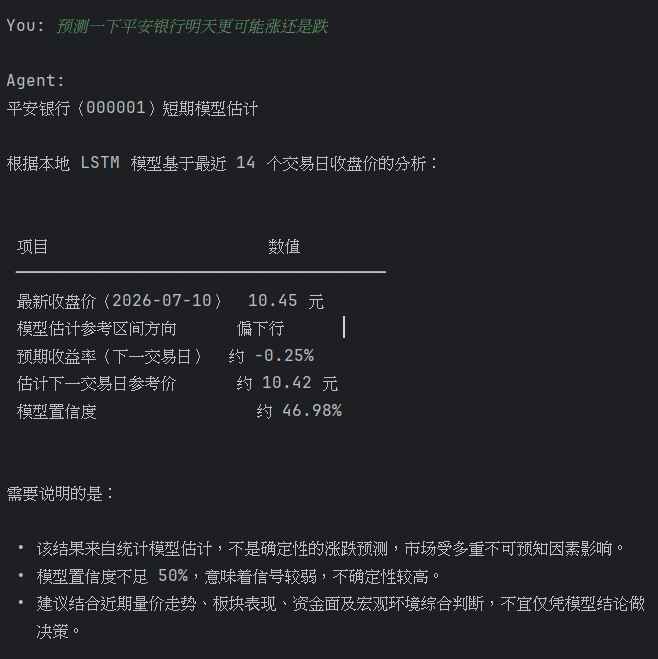
\includegraphics[height=0.72\textheight]{images/2026-07-12-15-40-07.png}
  \vspace{0.4em}

  \scriptsize\color{AccentGray}
  该回答由 \code{predict\_short\_term\_price} 生成：模型只给出短期统计参考，并明确提示不能替代综合投资判断。
\end{frame}

\begin{frame}{Agent 示例：深度研究报告节选}
  \scriptsize
  \begin{columns}[T]
    \begin{column}{0.49\textwidth}
      \begin{hlbox}[title=输入与综合结论]
        \textbf{问题：} 帮我深度分析一下贵州茅台的投资价值\\[0.25em]
        \textbf{综合评级：} 观望（Watch）\\
        \textbf{综合评分：} 54/100，置信度 45\%\\
        \textbf{仓位建议：} 0\%，保持观望
      \end{hlbox}
      \vspace{0.45em}
      \begin{greenbox}[title=基本面]
        PE(TTM) 18.21，合理偏低；PB 5.56，白酒龙头可接受；ROE 10.06\%，盈利稳健；资产负债率 12.12\%，财务安全。
      \end{greenbox}
      \vspace{0.45em}
      \begin{orangebox}[title=技术面与 LSTM]
        近 20 日涨幅 -3.68\%，RSI(14) 47.86，量比 0.80；LSTM 预期收益 -0.16\%，短期趋势偏弱。
      \end{orangebox}
    \end{column}
    \begin{column}{0.49\textwidth}
      \begin{hlbox}[title=新闻与情绪]
        新闻面：超 10 亿元回购计划，偏正面但强度一般。\\
        情绪面：百度情绪得分 -26，东方财富热度第 10，分歧与拥挤并存。
      \end{hlbox}
      \vspace{0.45em}
      \begin{greenbox}[title=风险提示]
        近 20 日弱势、缩量运行；散户情绪偏空；增长催化不足；LSTM 短期统计结果偏负。
      \end{greenbox}
      \vspace{0.45em}
      \begin{orangebox}[title=失效条件]
        高严重度负面新闻、跌破支撑并放量、盈利恶化或估值大幅提升时，评级需要下调；若回购落地并放量突破，可转为关注。
      \end{orangebox}
    \end{column}
  \end{columns}
  \vspace{0.45em}
  \centering
  \scriptsize\color{AccentGray}
  深度研究报告由 \code{run\_deep\_research} 汇总量化、基本面、新闻、情绪和 CIO 风控规则生成。
\end{frame}

\section{改进计划}

\begin{frame}{阶段问题与改进方向}
  \vspace{0.5em}
  \begin{orangebox}[title=LSTM 课程部分]
    \footnotesize
    只看 14 天收盘价信息量不足，模型增量信号较弱；下一步需要引入成交量、指数、行业、资金流等外生特征，让预测工具输出更有解释性的技术面参考。
  \end{orangebox}
  \vspace{0.9em}
  \begin{hlbox}[title=投资助手 Agent 部分]
    \footnotesize
    工具已经覆盖行情、财务、技术、宏观、筛选、回测与深度研究；下一阶段重点是做现实性测试：固定问题集、固定股票池、记录每日结果，并分析工具调用是否稳定、回答是否可复盘。
  \end{hlbox}
  \vspace{0.9em}
  \begin{greenbox}[title=需要继续加强]
    \footnotesize
    新闻/公告时间截断、外部接口稳定性、投资建议中的事实/模型/风险分层，以及长期测试样本的统计分析。
  \end{greenbox}
\end{frame}

\begin{frame}{后续计划与分工}
  \vspace{0.3em}
  \begin{hlbox}[title=统一收尾路线]
    \footnotesize
    \begin{itemize}
      \item 为价格模型继续补充成交量、指数、行业、资金流等外生特征
      \item 开始现实性测试：每天固定股票池，记录预测涨跌、工具调用和后续真实结果
      \item 统计预测命中率、收益回撤、失败案例，并用结果反向优化工具与提示词
    \end{itemize}
  \end{hlbox}
  \vspace{0.7em}
  \begin{greenbox}[title=分工安排]
    \footnotesize
    \centering
    \renewcommand{\arraystretch}{1.4}
    \setlength{\tabcolsep}{10pt}
    \begin{tabular}{lll}
      \toprule
      \textbf{成员} & \textbf{学号} & \textbf{负责内容} \\
      \midrule
      王昱人 & 3230105943 & Agent 架构设计与实现 \\
      高烁斌 & 3230101940 & Agent 测试、数据集测试、PPT 制作 \\
      于臻   & 3230105913 & LSTM 模型训练与优化 \\

      \bottomrule
    \end{tabular}
  \end{greenbox}
  \vspace{0.6em}
  \begin{center}
    {\kaifont\large\bfseries\color{ZJUBlue}最终目标：实现一个可用的 A 股预测 Agent}
  \end{center}
\end{frame}

\begin{frame}[plain]
  \vfill
  \begin{center}
    \begin{tikzpicture}
      \node[fill=ZJUBlue,text=white,minimum width=0.72\paperwidth,
            minimum height=3.2cm,inner sep=10pt,align=center] {
        {\kaifont\Huge\bfseries 谢谢聆听}\\[0.55em]
        {\Large 敬请批评指正}
      };
    \end{tikzpicture}
  \end{center}
  \vfill
  \begin{center}
    \small\color{AccentGray}
    克劳德老师，我还记得你 \quad | \quad A股预测 Agent
  \end{center}
  \vfill
\end{frame}

\end{document}
